% !TEX root = ../Rulebook.tex

Each of the particular tests defined later in this document may define its own scenario. In this document, a scenario consists of the following elements:

\begin{itemize}
	\item the environment
	\item the objects that affect navigation
	\item the objects that are to be manipulated
	\item the objects with which robots interact
	\item the number of robots allowed per team
	\item the number of teams competing simultaneously in the same arena
	\item the task to be performed by a team
	\item the criteria for evaluating a team's performance
\end{itemize}

In order to avoid excessive development efforts for each specific test and to allow reuse of partial functionalities the scenarios are built from a reasonably small set of components, which are later put together in different ways. This section describes these elements.

\section{Assumptions about Robots used in the Competition} \label{sec:AssumptionsAboutRobots}

The following assumptions are made about the kind of robots used in the competition:

\begin{itemize}

	\item At least one of the robots used by a team is mobile and moves on wheels. No specific assumptions are made about the kinematic design, but the mobile robots should be able to move on basically flat, sufficiently firm surfaces.
	\item The robots have at least one manipulator and are able to grasp objects, which are graspable by a parallel gripper with a jaw width of at least 5 cm and do not weigh more than 300 g.
	\item The robots use sensors to obtain information about their whereabouts in the environment and the task-relevant objects. The major types of sensors that may be used by the robots include:
	\begin{itemize}
		\item laser range finders (cf. models by Hokuyo or Sick)
		\item color CCD cameras (cf. any kind of USB camera)
		\item 3D cameras (such as the Kinect camera)
	\end{itemize}

	\item The design of the scenario should be such that the robots can solve the 	tasks safely and robustly using (all or a subset of) these sensors.

\end{itemize}



Future competitions may foresee the use of RFID sensors in the scenario design.


\section{Rules Applying to Robots} \label{sec:Robots}
The robots used for competition shall satisfy professional quality standards. The concrete definition of these standards is to be assessed by the TC, comprising aspects such as sturdy construction, general safety, and robust operation. It is not required that the robots are certified for industrial use.

\subsection{Robot Design and Design Constraints} \label{ssec:RobotDesignAndConstraints}
The robots need to comply with certain size constraints. A robot, including all parts attached to it as used in the competition, must be able to move by itself into a configuration so that it fits into a cube of side lengths 80 cm x 50 cm x 80 cm (length x width x height). If all the robot's parts, such as manipulator or anything able to protrude outside of the previously specified cube, are fully extended, the system must still not exceed a cube of side lengths 120 cm x 80 cm x 160 cm (length x width x height). The organizers may specify further constraints, such as weight limits. If a team would like to apply a robot with deviating robot dimensions, it should contact the TC. Exceptions for specific robots are possible in case of small differences.

\par
The manipulator of the robot should be designed and mounted on the robot such that it can grasp objects which will be placed in heights of between 0 cm and 40 cm above the floor.
\par
Electric, pneumatic, and hydraulic actuation mechanisms are permitted, provided that they are constructed and produced according to professional standards and meet safety constraints. Combustion engines and any kind of explosives are strictly forbidden. Robots may not pollute or harm their environment in any way, e.g. by loss of chemicals or oil, spilling liquids, or exhausting gases. Furthermore, constraints on the noise generated by a robot in operation may apply. These will be communicated in due time.
\par
If there are even vague doubts about the eligibility of using particular designs, parts, or mechanisms, the team should consult the TC well in advance.
\par
The robots have to be marked such that a clear distinction of robots used by different teams during a test is possible for spectators. The OC can define the concrete types of markers to be used. In this case the markers are not taken into account when checking the robot's size constraints. The markers shall not interfere with safe operation of the robot.
\par
The TC may require that robots are equipped with a wireless communication device of some sort (e.g. 802.11n), in order to communicate task specifications to the robots.

\subsection{Robot Behavior and Safety} \label{ssec:RobotBehaviorAndSafety}
In general, all robots shall be operated with maximum safety in mind. Any robot operation must be such that a robot neither harms humans nor damages the environment. A team must choose the operating parameters of their robot, e.g. the motion velocities for a robot base or a manipulator, or the grasp forces of a gripper, such that it can guarantee the safe operation of their robots.
\par
All robots must have a mechanical mechanism for immediately stopping the robot in cases of emergency. This mechanism must be clearly visible and easily accessible. The OC may request the proof of a robot's safety (e.g. the correct operation of an emergency stop) anytime during the tournament and exclude teams that cannot satisfy safety requirements.
\par
When participating in a tournament, the team may operate the robot only in their own team area, in the arenas provided (possibly constrained by a schedule assigning periods of time for exclusive use of the arena by a team or a group of teams), and in any other areas designated by the organizers for robot operation. Any operation of robots outside of these areas, e.g. in public areas or emergency paths, require prior permission by the OC.

\section{Referee Box}
The TC shall provide a referee box that supports the evaluation of the competition. It applies the time measuring, generates the tasks according to the chosen test configuration and monitors the
competition. For this purpose each robot has to transmit a keep-alive signal every second during all phases (initialization, preparation, game, finish). 

The referee box
\begin{enumerate}
  \item announces the start of the preparation time,
  \item communicates the task specifications,
  \item starts each competition run and
  \item closes a successful run after reaching the endzone or
  \item aborts the run in case of a time lapse.
\end{enumerate}

% Figure \ref{fig:refbox} depicts the progress of a competition run. 
When the robot is initialized, it starts immediately to transmit its beacon 
signal. The referee box answers with a state information. If the previous robot 
has left the arena, one of the referees starts the seconded phase by pushing a 
button. The referee box transmits a new state message that informs the robot 
about the beginning of the initialization phase. Inside the referee box a 
timer is started which initiates the start of the execution phase after 
transmitting the test parameters. During the run the robot is able to activate 
the external devices and to receive their status information. This run phase is 
terminated by a second timer that alerts after the duration defined in the 
instance table.
% 
% \begin{figure}
% \centering
% \begin{tikzpicture}[->,>=stealth',shorten >=1pt,auto,node distance=2.3cm,text centered, font={\footnotesize} ]
    \tikzstyle{element} = [draw=black, fill=white, rectangle, text width = 1.5cm, text centered, minimum height = 0.8cm, minimum width = 1.6cm]

    \tikzstyle{text_element} = [text width = 1.5cm, text centered]
    
    \node (ROBOT)[element]{@Work Robot};
    \node (REFBOX)[element, right of=ROBOT, fill=white, draw=black]{Refbox};
   \node (ROUNDTABLE)[element, right of=REFBOX]{Round Table};
  \node (CONVEYOR)[element, right of=ROUNDTABLE, fill=white, draw=black]{Conveyor Belt};
  
\coordinate (BELOW) at ($(ROBOT)+(0,-7.2cm)$);
\draw [dotted, -] (ROBOT) -- (ROBOT|-BELOW) ;
\draw [dotted, -] (REFBOX) -- (REFBOX|-BELOW) ;
\draw [dotted, -] (ROUNDTABLE) -- (ROUNDTABLE|-BELOW) ;
\draw [dotted, -] (CONVEYOR) -- (CONVEYOR|-BELOW) ;

\def \dist {1.0cm}
\coordinate (BEACON) at ($(ROBOT)+(0,-\dist)$);
\draw[->, dashed, gray] (BEACON) -- (BEACON-|REFBOX) node [midway] {{\tt beacon} } node [at end, anchor=center] (AUX){};

\def \dist {0.2cm}
\coordinate (START) at ($(AUX)+(0,-\dist)$);
\draw[->, blue] (START) -- (START-|ROBOT) node [midway] {{\tt gamestate} } node [at end, anchor=center] (AUX_1){};

\foreach \y in {2,...,6} 
       {\pgfmathtruncatemacro{\offset}{ \y * 1.3}
      \coordinate (BEACON) at ($(ROBOT)+(0,-\y)$);
       \draw[->, dashed, gray] (BEACON) -- (BEACON-|REFBOX) node [midway] {} node [at end, anchor=center] (AUX){};
} 

\def \dist {1.4cm}
\coordinate (START_PREP) at ($(START)+(0,-\dist)$);
\draw[->, blue] (START_PREP) -- (START_PREP-|ROBOT) node [midway, above] {{\tt gamestate}} node [at end, anchor=center] (AUX_1){};

\draw[-,decorate,decoration={brace,amplitude=5pt}] ($(START_PREP)-(2.5cm,-0.1cm)$) -- ($(START)-(2.5cm,0)$) node[midway, xshift=-0.3cm]{Initialisation};

\def \dist {0.3cm}
\coordinate (TASK) at ($(START_PREP)+(0,-\dist)$);
\draw[->] (TASK) -- (TASK-|ROBOT) node [midway] {{\tt taskinfo} } node [at end, anchor=center] (AUX_1){};

\def \dist {2.4cm}
\coordinate (START_GAME) at ($(START)+(0,-\dist)$);
\draw[->, blue] (START_GAME) -- (START_GAME-|ROBOT) node [midway] { {\tt gamestate} } node [at end, anchor=center] (AUX_1){};

\draw[-,decorate,decoration={brace,amplitude=5pt}] ($(START_GAME)-(2.5cm,-0.1cm)$) -- ($(START_PREP)-(2.5cm,0)$) node[midway, xshift=-0.3cm]{Preparation};

\draw[-, ultra thick] (START_PREP) -- (START_GAME) node [midway] {2 min};

\def \dist {5.4cm}
\coordinate (END_GAME) at ($(START)+(0,-\dist)$);
\draw[->,blue] (END_GAME) -- (END_GAME-|ROBOT) node [midway] { {\tt gamestate} } node [at end, anchor=center] (AUX_2){};

\draw[-,decorate,decoration={brace,amplitude=5pt}] ($(END_GAME)-(2.5cm,-0.1cm)$) -- ($(START_GAME)-(2.5cm,0)$) node[midway, xshift=-0.3cm]{Test execution};

\def \dist {0.9cm}
\coordinate (START_BELT) at ($(AUX_1)+(0,-\dist)$);
\draw[->] (START_BELT) -- (START_BELT-|ROUNDTABLE) node [midway, xshift=1cm] { {\tt command } } node [at end, anchor=center] (AUX_3){};

\def \dist {0.2cm}
\coordinate (END_BELT) at ($(AUX_3)+(0,-\dist)$);
\draw[->] (END_BELT) -- (END_BELT-|ROBOT) node [midway, xshift=1cm] { {\tt status } } node [at end, anchor=center] (AUX_1){};

\def \dist {0.9cm}
\coordinate (START_BELT) at ($(AUX_1)+(0,-\dist)$);
\draw[->] (START_BELT) -- (START_BELT-|CONVEYOR) node [midway, xshift=2cm] { {\tt command } } node [at end, anchor=center] (AUX_3){};

\def \dist {0.2cm}
\coordinate (END_BELT) at ($(AUX_3)+(0,-\dist)$);
\draw[->] (END_BELT) -- (END_BELT-|ROBOT) node [midway, xshift=2cm] { {\tt status } } node [at end, anchor=center] (AUX_1){};


\draw[-, ultra thick] (START_GAME) -- (END_GAME) node [midway, yshift=-1cm] {10min};

\end{tikzpicture}
% \caption{Sequence diagram of a complete competition run monitored by the referee box}
% \label{fig:refbox}
% \end{figure}
% \par
The TC provides a ROS and a MQTT based interface of the referee box as well as 
an reference implementation, that is available for all teams in February 2016.
The Referee box implementation and its documentation is available under the following link:
\begin{center}
	\url{www.google.de} \todo{specify correct URL}
\end{center}



% The publish/subscribe communication with the referee box and the external 
% devices have to be mapped on the following topics:\note{We should not talk about @Work being a game, e.g. "gamestate". (Sven and Fred)}

% \begin{table}[h!]
% \centering
%  \begin{tabular}{|l|c|c|p{5.9cm}|}
%  \hline
%  Topic & Robot & Refbox & Remarks \\ \hline\hline
%  {\tt /atwork/refbox/gamestate} & S & P & {\tt uint8 gamestate \newline
% uint8 PREPERATION  = 0\newline
% uint8 RUNNING\_TASK = 1\newline
% uint8 PAUSE    = 2  \newline
% uint8 END\_TASK     = 3\newline
% uint8 STOP     = 4 }\\ \hline
%   {\tt /atwork/refbox/beacon} & P & S & {\tt
%   geometry\_msgs/Pose2D position \newline
% string  current\_action } \\ \hline
%    {\tt /atwork/refbox/taskinfo } & S & P & {\tt BNT[] bnt\_tasks \newline
% BMT[] bmt\_tasks  \newline
% BTT[] btt\_tasks } \\ \hline
%    {\tt /atwork/refbox/[device]/command} & P & S & {\tt int8 state \newline
% int8 ERROR        = -1 \newline
% int8 NOT\_RUNNING  = 0 \newline
% int8 RUNNING      = 1   }\\\hline
%    {\tt /atwork/refbox/[device]/status  } & S & P & {\tt int8 state \newline
% int8 ERROR        = -1 \newline
% int8 NOT\_RUNNING  = 0 \newline
% int8 RUNNING      = 1   }\\\hline
%  \end{tabular}
%   \label{tab:RefBoxTopics}
%  \caption{Referee box topics}
% \end{table}
% 
% \begin{table}[h!]
% \centering
%  \begin{tabular}{|l|p{6.3cm}|}
%  \hline
%  Message types & Remarks \\ \hline\hline
%  {\tt Atworkobject} & {\tt uint8 name\newline
% uint8 F20\_20\_B = 0 \newline
% uint8 F20\_20\_G = 1 \newline
% uint8 S40\_40\_B = 2 \newline
% uint8 S40\_40\_G = 3 \newline
% uint8 M20\_100  = 4 \newline
% uint8 M20      = 5 \newline
% uint8 M30      = 6 \newline
% uint8 R20      = 7 \newline
% \revdel{uint8 V20      = 8} \newline
% string destination }\\ \hline
% 
%  {\tt BNT} &  {\tt Waypoint[] waypoints }\\ \hline
% 
%  {\tt BMT} &  {\tt string   startplace \newline
% string[] pickObjects \newline
% string   destination }\\ \hline
% 
%   {\tt BTT} &  {\tt string destination  \newline
% AtworkObject[] objects }\\ \hline
%    {\tt Waypoint  } &  {\tt string position \newline
% uint8  orientation \newline
% uint8  WEST  = 0 \newline
% uint8  EAST  = 1 \newline
% uint8  SOUTH = 2 \newline
% uint8  NORTH = 3 \newline
% uint32  duration  }\\\hline
%  \end{tabular}
%  \caption{Refere box auxiliary message types \todo{can we provide a repository where the message files are stored? And make it consistent with items in Table \ref{tab:manipulation_objects} and \ref{tab:manipulation_objects_rockin}. And add the missing test like PPT, CBT, etc.}}
%   \label{tab:RefBoxAUX}
% \end{table}
% 
% Table~\ref{tab:RefBoxAUX} summarizes the auxiliary types embedded in
% the referee box messages. A detailed description of the referee box-API is given in the 
% corresponding documentation available on \todo{???????????????}. 

\par
The referee box visualizes the current state of the competition run, \revdel{current} time measurements, the task specification and robot positions for visitors. Team information (name, affiliation, contact information) are given too in this context.

\todo{NICO: add maybe some screenshots from the referee box, also make a reference to the FESTO referee box}

\section{Use of External/Control Devices}
No external devices are allowed (e.g. remote controls) in general. Exceptions may be certain simplifications leading to reduction of points as described in Section~\ref{ssec:ScoringAndRanking}, or in particular tests. All communication of the robots with external elements must be wireless. Cable connections between the robot and external devices are not allowed during competition runs.
\par
%  It is possible for the TC to choose an alternative referee box software, or to allow teams to use their own referee box. This must be announced before the tournament starts.
A team may set up an additional external computer to monitor the operation of their robot(s) during a run. This monitoring system must be designed such that no manual interaction through keyboard, mouse, or any other input device is required during a run. Team members must keep their hands off the keyboards and mice of all their computers during a run.
It must be clear at all times that no manual or remote control is exerted to influence the behavior of the robots during a run. Exceptions may be specified by particular tests, e.g. for tasks where handing over objects to humans is required.

\section{Design of Competition Arenas}
\label{sec:ArenaDesign}
\subsection{Size of the Arena}

The size of a competition arena is a rectangular area not lesser than 2 m x 4 m and not more than 10 m x 12 m.
An orientation is always associated with the arena. An arbitrary wall is designated as “North” orientation, and the wall to its right is designated as “East” and so on. The orientations will be assigned by the local league chair or/and the TC as soon as the arena is built up. Figure~\ref{fig:example_arena} shows one possible example of an arena configuration, while Figure~\ref{fig:example_topological_map} illustrates the topology.

\begin{figure}

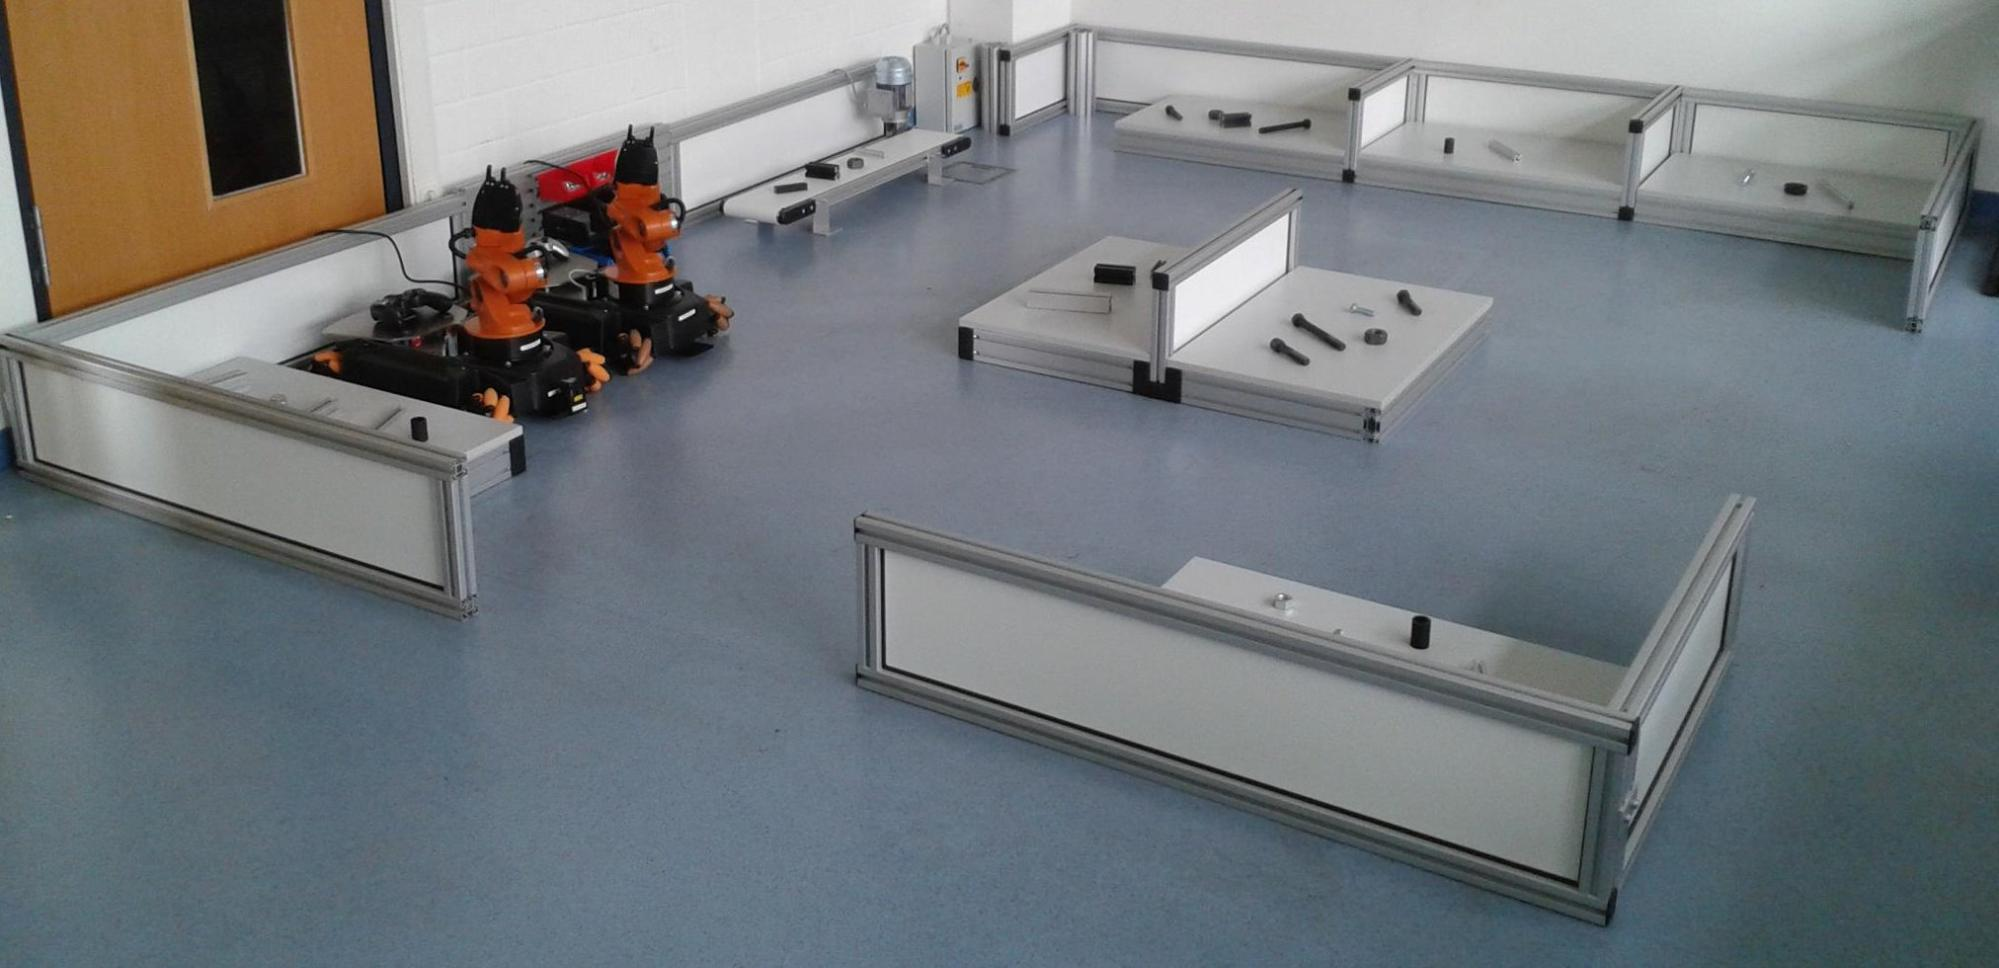
\includegraphics[width= \textwidth ]{./images/example_arena.jpg}
\caption{An exemplary setup of a \RCAW environment.}
\label{fig:example_arena}
\end{figure}

\begin{figure}
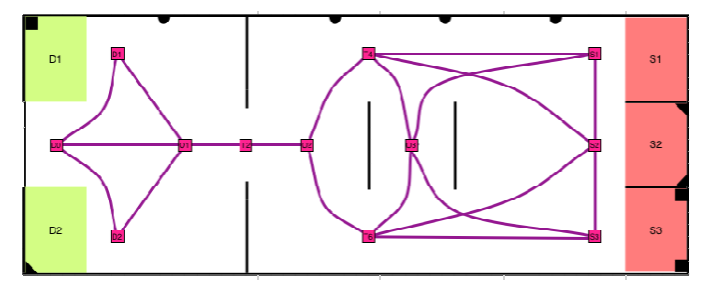
\includegraphics[width= \textwidth ]{./images/example_map.png}
\caption{Topological map with five service areas (D1, D2, S1, S2, S3). The purple squares define places.}
\label{fig:example_topological_map}
\end{figure}


\subsection{Floor}
The floor is made of some firm material. Examples include floors made of concrete, screed, timber, plywood, chipboard, laminated boards, linoleum, PVC flooring, or carpet. Some examples are illustrated in Figure \ref{example_floors}. Floors may neither be made of loose material of any kind (gravel, sand, or any material which may damage the functioning of the robots' wheels) nor may such material be used on top of the floor. Liquids of any kind are not allowed. The floor may have spots of unevenness of up to 1cm in any direction (clefts, rifts, ridges, etc.).

\begin{figure}
\begin{center}
\subfloat[]{
\includegraphics[height = 2cm]{./images/example_floor_1.jpg}}
\subfloat[]{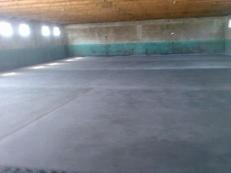
\includegraphics[height = 2cm]{./images/example_floor_2.jpg}}
\subfloat[]{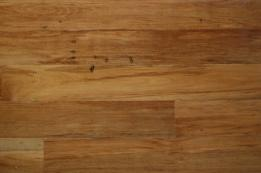
\includegraphics[height = 2cm]{./images/example_floor_3.jpg}}
\subfloat[]{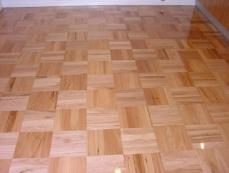
\includegraphics[height = 2cm]{./images/example_floor_4.jpg}}
\subfloat[]{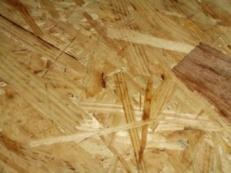
\includegraphics[height = 2cm]{./images/example_floor_5.jpg}}\\
\subfloat[]{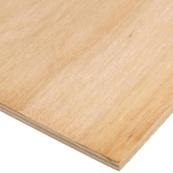
\includegraphics[height = 2cm]{./images/example_floor_6.jpg}}
\subfloat[]{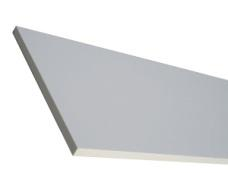
\includegraphics[height = 2cm]{./images/example_floor_7.jpg}}
\subfloat[]{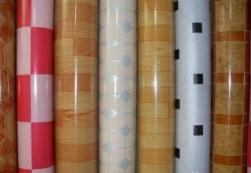
\includegraphics[height = 2cm]{./images/example_floor_8.jpg}}
\subfloat[]{
\includegraphics[height = 2cm]{./images/example_floor_9.jpg}}
\subfloat[]{
\includegraphics[height = 2cm]{./images/example_floor_10.jpg}}
\end{center}

\caption{Examples of floors that can be used for \RCAW arenas.}
\label{example_floors}
\end{figure}

\subsection{Walls}
The competition arena is partially surrounded by walls. The height of the walls is not lesser than 20 cm and not more than 40 cm. One or more gates may be foreseen, where robots can enter or leave the arena. Gates may or may not be closable. The walls have a mostly uniform color. Small visual elements like logos or advertisements may be placed on the walls.

\subsection{Service Areas}
Arenas contain one or more service areas, which have specific purposes for a particular test. Examples include loading and unloading areas, conveyor belts, rotators, storage areas, etc. Service areas may contain specific environment objects, such as racks, shelves, etc. They may be accessible from different locations, i.e. it might be possible to reach an area from two or more sides.

\subsection{Racks}
Service areas, e.g. loading and unloading areas, may foresee the use of racks. Objects to be delivered or removed from racks have to be placed or picked up from the top. The height of the racks should be not lesser than 5 cm and not more than 40 cm. The color for the top surface of racks is a bright uniform color such as white or light gray, unless a test specifies a different color. The top surface of the rack may be specially designed in order to serve specific purposes, e.g. holding objects.

\subsection{Shelves}
Service areas may foresee the use of shelves and shelf units. Objects to be delivered or removed from shelves have to be placed or picked sideways. The height of the shelves should be not lesser than 5 cm and not more than 40 cm. The color of the shelf surface is a bright uniform color such as white or light gray, unless a test specifies a different color. The shelf surface may be specially designed in order to serve specific purposes, e.g. holding objects.

\subsection{Places}
An arena designed for a particular test may foresee the definition of a set of designated places, which are locations in the arena that can be referred to by a unique, symbolic identifier. These identifiers are used e.g. for the task specification, possibly in conjunction with other information, such as an orientation. Places may be marked by markers of some sort.

\subsection{Obstacles}
An arena defined for a particular test may foresee the use of obstacles. Obstacles may by passive (i.e. not able to relocate by themselves) or active (e.g. other robots). The size of obstacles should be not lesser than 10 cm x 10 cm x 5 cm; there is no upper bound on the size. The details about the dynamic objects are not known before the competition and will be chosen by the OC on-site. Examples for obstacles are trash bins, boxes, big aluminium profiles or even other robots.

\subsection{Floor Markers}
The arena used for a particular test may foresee the use of floor markers for designated places. The design of these floor markers are rectangular black-and-white images as used by the ARToolKit library:
\begin{center}
\url{http://www.hitl.washington.edu/artoolkit}
\end{center}

The black inner square of the markers is at least 8 cm x 8 cm large with an additional white border around of at least 12 cm side length. Figure \ref{fig:floor_marker} and \ref{fig:barrier_tape} depict some examples of these markers.

\begin{figure}
\centering

\includegraphics[width= 0.4\textwidth ]{./images/example_floor_marker.png}
\caption{Example of a floor marker.}
\label{fig:floor_marker}
\end{figure}


\subsection{Barrier Tape as Virtual Walls}
The arena may include virtual walls marked by either striped yellow/black or white/red barrier tape on the floor (see Figure \ref{fig:barrier_tape}). If any part of a robot passes over such a tape it is considered as a collision with a usual wall.

The red/white tape is used to frame the entrance and exit area. The robot is allowed to cross this kind of barrier only at the beginning of a test to enter arena and at the end for leaving. In contrast, the yellow/black one denotes an obstacle which the robot is never allowed to cross. 

\begin{figure}
\centering
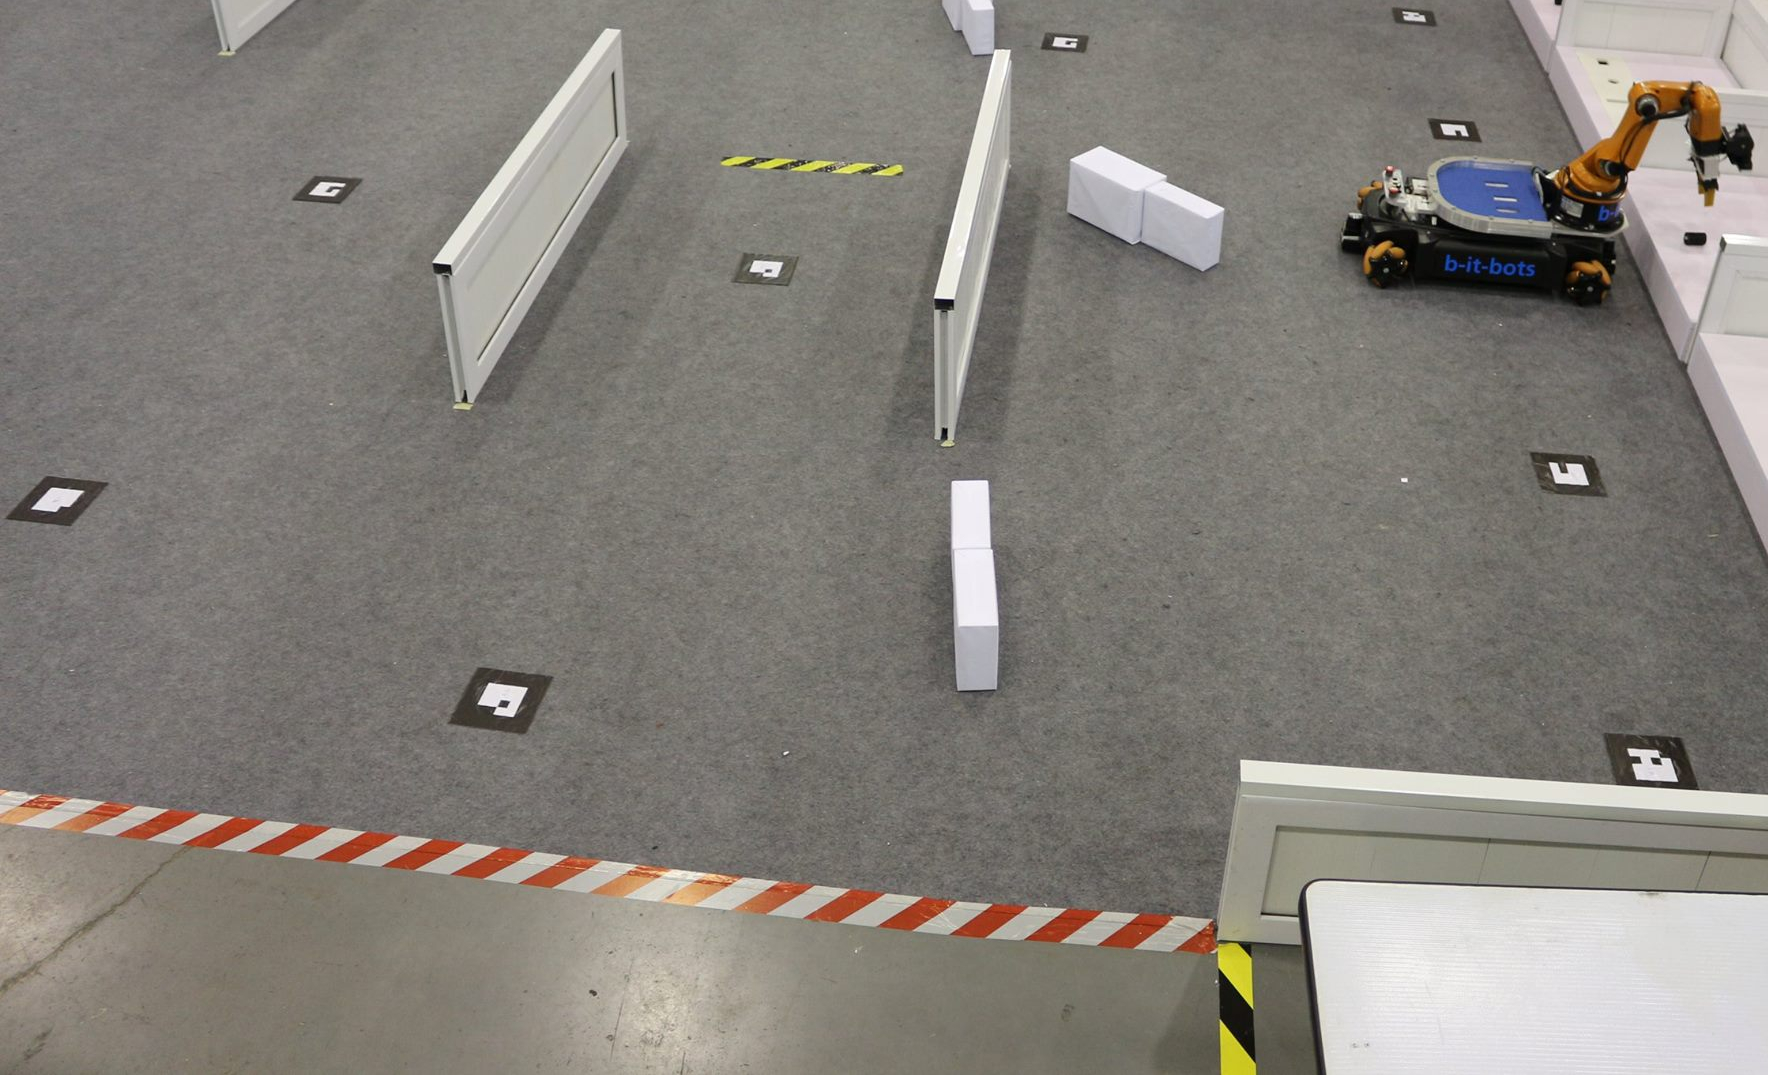
\includegraphics[width= 0.7\textwidth ]{./images/barrier_tapes_in_china15.jpg}
\caption{Example of barrier tape used during \RC 2015. The red/white tape is used for the entrance and exit, while the yellow/black one denotes an obstacle.}
\label{fig:barrier_tape}
\end{figure}


\subsection{Entrance and Exit}
If possible, the arena should have one entrance and one exit, which are equipped with laser barriers. These barriers are used for timekeeping by the referee box.

\subsection{Setup of the Arena}
The arena must be surrounded by either walls or barrier tape. The only exceptions are the entrance and exit. There must be a route to all places and markers relevant for a test which has a minimum width of 55 cm.

\section{Design of Manipulation Tasks}
\label{sec:ManipulationTasks}

\subsection{Manipulation Objects} \label{ssec:ManipulationObjects}
The manipulation objects in \RCAW shall include a wide range of objects relevant in industrial applications of robotics. They eventually cover any raw material, (semi-)finished parts or products as well as tools and possibly operating materials required for manufacturing processes.
\par
The intention is to start with a simple set of objects of different shapes and colors. Every year, the spectrum shall then be widen in at least one aspect. The initial set of objects includes basic standard screws and nuts in various sizes and weights as shown in Table~\ref{tab:manipulation_objects} and Table~\ref{tab:manipulation_objects_rockin}. Objects of one kind can slightly vary e.g. considering the surface. 

\newcommand{\imageView}[1]{\includegraphics[width=2cm, valign=c]{#1}}
{
\newcommand{\rowpadding}{0.4cm}
\setlength\extrarowheight{\rowpadding}
\begin{table}[p]
\begin{tabular}{|c|c|c|m{6cm}|}
\hline
Object & Symbolic Description & Weight & Details \\
\hline
\imageView{./images/F20_20_B.jpg} & \texttt{F20\_20\_B} & 49 g & Small aluminium profile (black)\newline
 Height: 20 mm \newline
 Width: 20 mm \newline
 Length: 100 mm \\ [\rowpadding]
\hline
\imageView{./images/F20_20_G.jpg} & \texttt{F20\_20\_G} & 49 g & Small aluminium profile (gray)\newline
 Height: 20 mm \newline
 Width: 20 mm \newline
 Length: 100 mm \\ [\rowpadding]
\hline
\imageView{./images/S40_40_B.jpg} & \texttt{S40\_40\_B} & 186 g & Big aluminium profile (black)\newline
 Height: 40 mm \newline
 Width: 40 mm \newline
 Length: 100 mm \\ [\rowpadding]
\hline
\imageView{./images/S40_40_G.jpg} & \texttt{S40\_40\_G} & 186 g & Big aluminium profile (gray)\newline
 Height: 40 mm \newline
 Width: 40 mm \newline
 Length: 100 mm \\ [\rowpadding]
\hline
\imageView{./images/M20_100.jpg} & \texttt{M20\_100} & 296 g & Screw\newline
 ISO 4014 \newline
 M20 \newline
 Length: 100 mm \\ [\rowpadding]
\hline
\imageView{./images/M20.jpg} & \texttt{M20} & 56 g & Small nut\newline
 ISO 4032 \newline 
 M20 \\ [\rowpadding]
\hline
\imageView{./images/M30.jpg} & \texttt{M30} & 217 g & Big nut\newline
 ISO 4032 \newline 
 M30 \\ [\rowpadding]
\hline
\imageView{./images/R20.jpg} & \texttt{R20} & 14 g & Plastic tube\newline
 Inner diameter: 20 mm \newline
 Outer diameter: 30 mm \newline
 Length: 45 mm \\ [\rowpadding]
\hline
%\imageView{./images/V20.jpg} & \texttt{V20} & 14 g & Inner diameter: 20 mm \newline
%Outer diameter: 30 mm \newline
%Length: 45 mm \\
%\hline
\end{tabular}
\caption{\RCAW manipulation object set.}
\label{tab:manipulation_objects}
\end{table}


\begin{table}[p]
\begin{tabular}{|c|c|c|m{6cm}|}
\hline
Object & Symbolic Description & Weight & Details \\
\hline

\imageView{./images/bearingBoxA.jpg} & \texttt{Bearing\_Box} & 102 g & Bearing box\newline
 Height: 25 mm \newline
 Width: 45 mm \newline
 Length: 50 mm \newline
 Inner diameter: 32 mm \\ [\rowpadding]
\hline

\imageView{./images/bearing.jpg} & \texttt{Bearing} & 42 g & Bearing\newline
 Height: 13 mm \newline
 Inner diameter: 15 mm \newline
 Outer diameter: 32 mm \\ [\rowpadding]
\hline

\imageView{./images/axis.jpg} & \texttt{Axis} & 40 g & Axis\newline
 Diameter: 27 mm \newline
 Length: 96 mm \\ [\rowpadding]
\hline

\imageView{./images/distanceTube.jpg} & \texttt{Distance\_Tube} & 5 g & Distance tube\newline
 Height: 10 mm \newline
 Inner diameter: 28 mm \newline
 Outer diameter: 32 mm \\ [\rowpadding]
\hline

\imageView{./images/motor.jpg} & Motor & 20 g & Motor\newline
 Diameter: 42 mm \newline
 Length: 87 mm \\ [\rowpadding]
\hline
\end{tabular}
\caption{RoCKIn manipulation object set.}
\label{tab:manipulation_objects_rockin}
\end{table}
}

\subsection{Manipulation Zone}
The manipulation zone defines the area where objects can be placed. Thereby, the following constraints need to be satisfied:
\begin{itemize}
	\item The maximum depth of the manipulation zone is 20 cm.
	\item The minimum distance between objects to each other is 2 cm.
	\item The minimum distance of the beginning of the manipulation zone to a wall is 10 cm.
	\item There as an offset of 2 cm from the border of the service area to the manipulation zone.
\end{itemize}
Note, the constraints do not permit, that objects can be partially occluded dependent on the viewpoint.
\begin{figure} [h!]
\centering
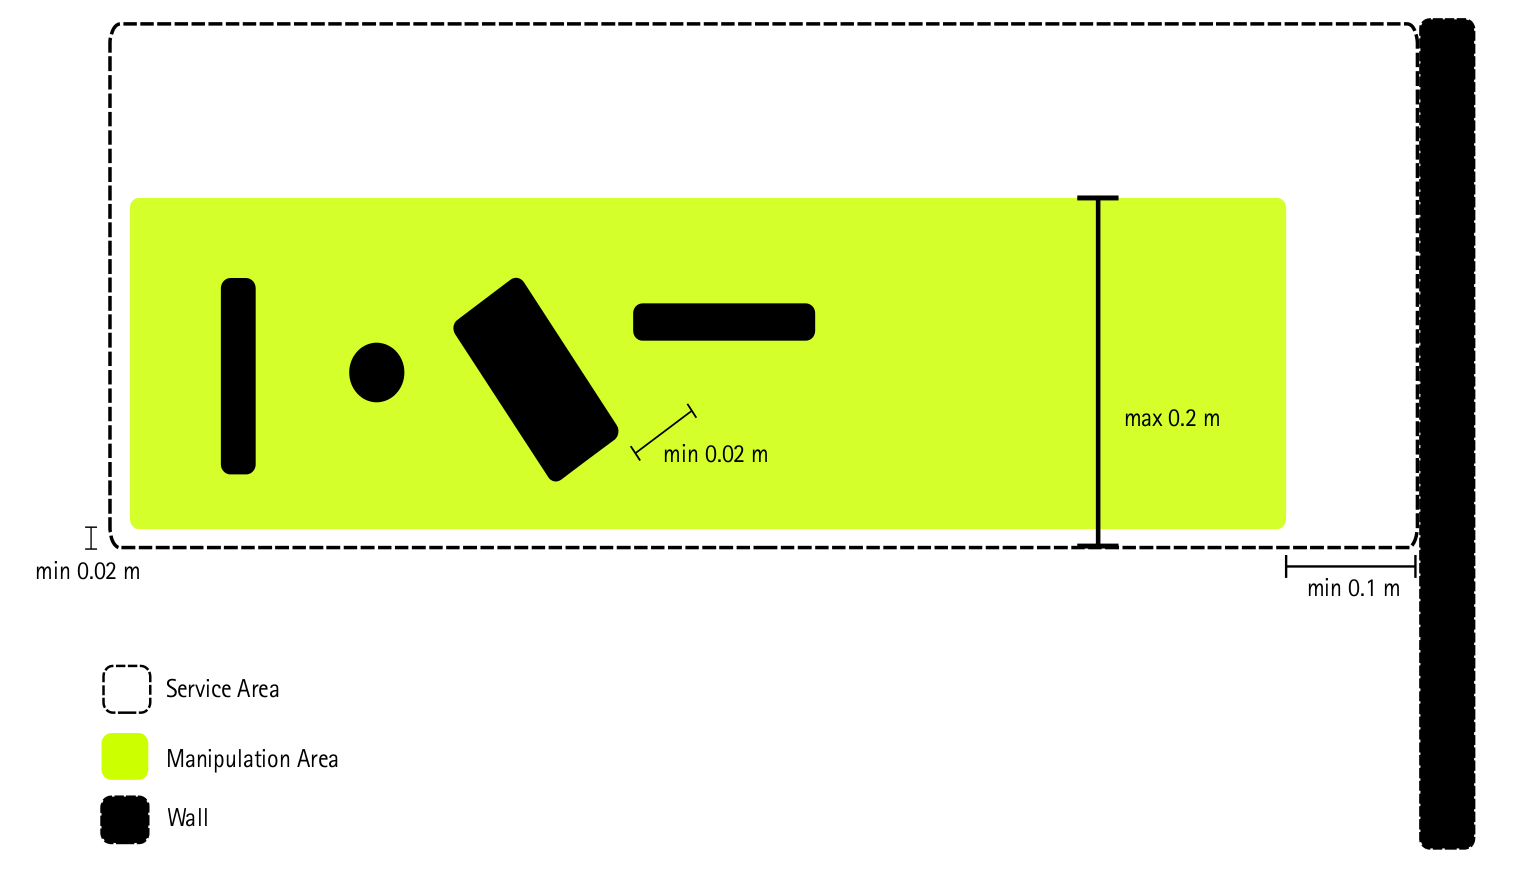
\includegraphics[width=1.0\textwidth ]{./images/manipulation_zone.png}
\caption{Manipulation zone: the green color indicates the area where objects can be placed on a service area by the referees.}
\label{fig:manipulation_zone}
\end{figure}





\subsection{Placement of Objects}
For the placement of manipulation objects the following terms are used:

\begin{itemize}
\item position: point within 2D coordinate system of a service area,
\item rotation: rotation around vertical axis of a service area,
\item orientation: rotation around horizontal axes of a service area, i.e. whether the object is standing upright or lying on its side
\item pose: combination of position, rotation and orientation.
\end{itemize}

\subsection{Grasping Objects} \label{ssec:GraspingObjects}
If not specified differently in a test, the following definition applies to decide if an object counts as being grasped from a service area.
\par
An object counts as grasped from a service area, when the object was moved outside of the source service area. Outside means, that the vertical projection of the object’s convex hull does not touch the service area any more.

\par
The last point shall enable to let the robot pick up an object in order to analyse its type, e.g. by holding it close to a camera on the robot.
\par
If the robot handles an object, but does not fulfil all points above, the object does not count as being grasped, and neither points for grasping a required object, nor penalty points for grasping an unspecified object are given. Still, if the object drops to the ground or an uncontrolled collision occurs, the normal penalty points apply.

\subsection{Placing Objects on Service Areas} \label{ssec:PlacingObjects}
If not specified differently in a test, a manipulation object counts as placed on a target service area if any part of the object is touching the surface of the service area and the object is not moving at the end of the run.
\par
The pose of the object on the service area can be chosen freely by the robot.

%\section{Overall Scenario and Variation Points}
%The following two figures illustrate the kind of arenas that can be built with the previously described components. Figure \ref{fig:example_map} shows an old arena configuration (from IROS 2012) as a topological map defining places and connections, while Figure \ref{fig:example_map_go13} shows an arena configuration (from German Open 2013) with only a few surrounding walls, more open space and a conveyor belt. 

%\begin{figure}
%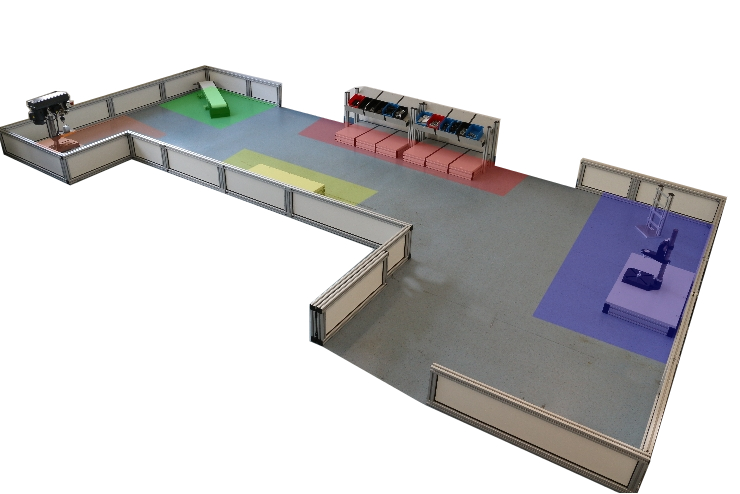
\includegraphics[width= \textwidth ]{./images/arena_brsu_spatial_areas.jpg}
%\caption{Illustration of one possible arena configuration. \todo{similar to Figure~\ref{fig:example_arena}. Delete one or put them together in a subfigure environment}}
%\label{fig:example_map_brsu}
%\end{figure}
